\documentclass[../main.tex]{subfiles}

\begin{document}

\newcommand{\flippedstep}[3]{
    \begin{tcolorbox}[
        boxrule=0pt, colframe=black!5,
        coltitle=black, colback=#1,
        step=sample,
        height=7.5cm
    ]
    \begin{center}
        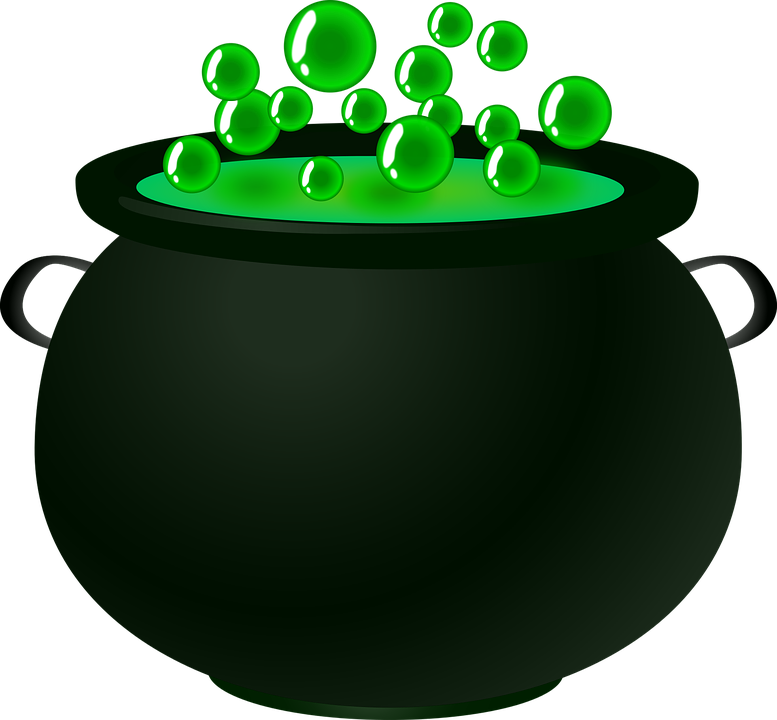
\includegraphics[height=3cm]{images/zaubertrank.png}
    \end{center}
    \tcblower
    \begin{center}
        \textbf{#2}
    \end{center}
    \scriptsize #3
    \end{tcolorbox}
}

\parpic[r]{
    \tikz[scale=1.9]{\sloth}
}
Bevor es mit der Mathematik losgeht, möchten wir gern noch ein paar Worte darüber verlieren, wie das Lernen mit diesem Buch und den Begleitmaterialien, die dafür erstellt worden sind, gedacht ist. Wir möchten außerdem das Lehrkonzept \emph{Flipped Classroom} genauer erläutern, damit du das beste für dich dabei herausholen kannst. Um dir nur das zu erklären, was für dich interessant ist, haben wir diese Einführung danach unterteilt, wer du bist und was deine Ziele sind, wenn du mit diesem Buch arbeitest. Wir gehen davon aus, dass auf dich einer der folgenden Punkte zutrifft.

\begin{enumerate}
    \item[\tikzball{blue!40}{1}] Du bist \textbf{Schüler} und dein Lehrer hat sich entschieden, dieses Buch für seinen Matheunterricht zu verwenden.
    \item[\tikzball{blue!40}{2}] Du bist \textbf{Lehrer} und möchtest unser Buch bei deiner Unterrichtsgestaltung verwenden.
    \item[\tikzball{blue!40}{3}] Du bist einfach so auf dieses Buch gestoßen und möchtest deine mathematischen Grundlagen festigen oder vertiefen.
\end{enumerate}

Wir haben uns überlegt, welche Ziele du haben könntest, wenn du mit dem Reiseführer arbeitest. Diese haben wir danach aufgeteilt, ob du Lehrer, Schüler oder vielleicht auch Student oder einfach nur interessiert bist. Für jedes Ziel, das uns eingefallen ist, haben wir einige Tipps aufgeschrieben, wie du es mit dem Reiseführer am besten erreichen kannst. 

Wenn du ein Schüler bist, dann gehen wir davon aus, dass dein Lehrer sich dafür entschieden hat, mit dem Reiseführer ein \emph{Flipped Classroom}-Konzept umzusetzen. Bist du dir nicht sicher, dann frage nochmal nach. Was das \emph{Flipped Classroom}-Konzept ist und wie du damit arbeiten kannst, erklären wir dir im Abschnitt \enquote{Lernen mit Flipped Classroom}. Den Abschnitt zum Aufbau dieses Buchs kannst du überspringen, da er für diejenigen gedacht ist, die mit diesem Buch lernen wollen, aber kein Flipped Classroom-Konzept verwenden.

Falls du ein Lehrer bist, empfehlen wir dir, alles durchzulesen, damit du die verschiedenen Arbeitsweisen, die wir empfehlen, kennst und dich auf sie einstellen kannst. Extra für Lehrer gibt es außerdem noch einen Abschnitt \enquote{Unterrichtsgestaltung mit dem Reiseführer Mathematik}.

\newpage
\section*{Aufbau dieses Buchs}
\label{concept}

Zum \emph{Reiseführer Mathematik} gehört nicht nur dieses Buch, sondern noch eine Reihe weiterer Materialien. Insgesamt besteht dieses Lehrwerk aus den folgenden Komponenten:
\begin{enumerate}
    \item[\tikzball{blue!40}{1}] diesem \textbf{Buch}, das Erklärungen zu den üblicherweise in der Schule behandelten Themen enthält
    \item[\tikzball{blue!40}{2}] pro Kapitel einem Satz \textbf{Vorbereitungsblätter}, die jeweils den Abschnitten dieses Buchs zugeordnet sind und eine Hilfestellung beim Durcharbeiten der entsprechenden Abschnitte sein sollen
    \item[\tikzball{blue!40}{3}] pro Kapitel einem \textbf{Aufgabenblock}, der Übungsaufgaben verschiedener Schwierigkeitsgrade sowie Beispiellösungen zu den Inhalten des entsprechenden Kapitels enthält
    \item[\tikzball{blue!40}{4}] \textbf{Erklärvideos}, die dieselben Inhalte wie das Buch behandeln
\end{enumerate}

Dieses Buch unterscheidet sich von den meisten Lehrbüchern, weil es keine Aufgaben enthält. Stattdessen kannst du in diesem Buch viele Beispiele und ausführlichere Erklärungen finden.

Jedes Kapitel in diesem Buch ist in verschiedene Abschnitte aufgeteilt (z.\,B. die Einführung). In diesen Abschnitten erklären wir dir das gerade behandelte Thema so, dass du es (ggf. mit dem Vorwissen aus den vorangegangenen Kapiteln) verstehen kannst. Dabei verwenden wir viele ausführliche Beispiele und Erklärungen. Du musst dir nicht unbedingt alle Beispiele genau durchlesen, wenn du dir zutraust, das Thema auch ohne sie zu verstehen. Alle Inhalte, die wichtig sind, werden im Text außerhalb der Beispiele so erklärt, dass du auch ohne die Beispiele verstehen kannst, worum es geht. 

Um dir später das Wiederholen der Inhalte zu erleichtern, endet jeder Abschnitt mit einer Zusammenfassungsbox wie der folgenden.

\begin{nutshell}{Zusammenfassungsboxen}
    Am Ende jedes Abschnitts in diesem Buch findest du eine Box wie diese. Hier werden alle wichtigen Erkenntnisse, die im Abschnitt vorkamen, genannt und knapp erklärt. Eine Zusammenfassungsbox enthält jedoch keine ausführlichen Erklärungen oder Beispiele. Mithilfe dieser Boxen kannst du einen guten Überblick über die Themen bekommen, wenn du sie bereits verstanden hast.
\end{nutshell}

\begin{advanced}{Weiterführendes Wissen}
    Zusätzlich zu den Inhalten, die für die Schulmathematik zwingend notwendig sind, enthält dieses Buch auch Einblicke in Themen, die darüber hinaus gehen. Falls die normalen Themen keine ausreichende Herausforderung für dich sind und du dich mit ein wenig komplizierteren Themen beschäftigen möchtest, dann solltest du nach den violett hinterlegten Teilen im Buch Ausschau halten. Diese befinden sich zum einen am Ende jedes Kapitels. Darüber hinaus findest du hin und wieder violett hinterlegte Blöcke wie diesen, die über die Kapitel verteilt auftauchen. Sie enthalten Ergänzungen zu dem Thema, über das du gerade etwas gelesen hast und verweisen manchmal auf die violetten Seiten am Ende des Kapitels.

    Die Inhalte dieser Blöcke sind für das restliche Buch nicht weiter wichtig. Du wirst immer in der Lage sein, das Buch zu verstehen, auch wenn du diese Boxen einfach ignorierst, weil es im Buch keine Stellen gibt, die auf weiterführendem Wissen aufbauen.
\end{advanced}

Weitere farbige Boxen, die du beim Lesen dieses Buchs immer wieder sehen wirst, sind die folgenden beiden.

\begin{definition}{}
    In Boxen wie dieser findest du Definitionen. Eine Definition ist eine Schreibweise oder ein Name, die sich Mathematiker für etwas ausgedacht haben, was sie häufig verwenden. Die neuen Begriffe, die wir in Definitionen einführen, machen uns das Leben einfacher, weil wir sie als eine Art Abkürzung für Dinge verwenden können, die wir sonst viel umständlicher aufschreiben müssten.
\end{definition}

\begin{theorem}{}
    Sätze sind eigentlich der spannendste Teil der Mathematik. Anders als Definitionen, in denen wir zwar neue Schreibweisen einführen, ist ein Satz eine Aussage, die immer gilt und die sich logisch aus dem, was wir bereits wissen, herleiten lässt.
\end{theorem}

Um dich beim Verstehen der Erklärungen aus dem Buch zu unterstützen, gibt es \textbf{Vorbereitungsblätter}. Jedes Vorbereitungsblatt gehört zu einem Abschnitt aus dem Buch. Zu allen Abschnitten, die du im Inhaltsverzeichnis sehen kannst, gehört also ein Vorbereitungsblatt. Die einzige Ausnahme sind die Abschnitte mit weiterführendem Wissen, die im Buch violett hinterlegt sind und zu denen kein Vorbereitungsblatt gehört.

Ein Vorbereitungsblatt enthält alle wichtigen Definitionen und Sätze aus dem Abschnitt im Buch, zu dem es gehört. Du kannst ein Vorbereitungsblatt als eine Art Anleitung zum Durcharbeiten des Buchs verwenden. Die Buchstellen, die für ein Vorbereitungsblatt wichtig sind, findest du in den grauen Kästen auf den Vorbereitungsblättern. Auf der linken Seite dieser Kästen findest du außerdem immer einen QR-Code, der zu einem Video führt, das die selben Inhalte erklärt. Du kannst dir also aussuchen, ob du die Inhalte lieber durch ein Video erklärt bekommen möchtest oder ob du sie dir lieber im Buch durchlesen möchtest.

\newtcolorbox{video}{code={\pgfkeysalsofrom{\tcmathenvopt}}, colback=black!10,colframe=black!30, boxsep=0pt}
\begin{video}
    \begin{minipage}{.1\textwidth}
        \qrcode[height=1cm]{https://themrsheldon.github.io/testing/}
    \end{minipage}
    \begin{minipage}{.9\textwidth}
        \href{https://themrsheldon.github.io/testing/}{\textbf{Video:} \textit{Beispiel-Video}} (5 Minuten)\\
        Aufbau dieses Buchs (ab Seite \pageref{concept})
    \end{minipage}
\end{video}

Während du die Videos schaust oder die Seiten im Buch durchliest, auf die das Vorbereitungsblatt verweist, kannst du mit den Verständnisfragen auf dem Vorbereitungsblatt prüfen, ob du verstanden hast, was du gerade gelesen oder gehört hast. Zu jedem Video gehört deshalb ein kleiner Aufgabenteil mit Aufgaben, die du schnell durch das Ausfüllen eines Lückentextes, durch Ankreuzen oder ähnliches beantworten kannst.

Um das Thema eines Abschnitts in diesem Buch besser zu verstehen und zu üben, kannst du die Übungsaufgaben bearbeiten, die in den \textbf{Aufgabenblöcken}, die es zu jedem Kapitel gibt, enthalten sind. Die Übungsaufgaben ergänzen die Aufgaben auf dem Vorbereitungsblatt und sind teilweise deutlich zeitaufwändiger. Sie unterteilen sich in verschiedene Schwierigkeitsstufen, die auf den Aufgabenblöcken genauer erklärt sind. Außerdem findest du auf den Aufgabenblöcken Beispiellösungen mit Erklärungen, die beschreiben, wie du an bestimmte Arten von Aufgaben herangehen kannst.

Falls du beim Bearbeiten von Aufgaben nicht weiterkommst, kannst du einen der Hinweise verwenden, die es zu den meisten Aufgaben gibt. Hinweise versuchen, dich in Richtung der Lösung zu lenken, ohne die Lösung dabei zu verraten. Schließlich endet jeder Aufgabenblock mit einem Selbsttest. Dieser besteht aus einer kleinen Sammlung von Aufgaben, die das gesamte Wissen des Kapitels voraussetzen und die du zum Beispiel als Vorbereitung auf eine Klausur rechnen kannst. Du solltest versuchen, diese Aufgaben ohne Hilfsmittel zu bearbeiten. Sie sind dafür ausgelegt, dass du sie in 90 Minuten lösen kannst.

\newpage

\section*{Lernen mit \enquote{Flipped Classroom}}
Im traditioneller Unterricht erklärt ein Lehrer seinen Schülern im Unterricht ein neues Thema, das anschließend geübt wird. Bei seiner Erklärung kann er jedoch unmöglich auf alle einzelnen Schüler in seiner Klasse gleichzeitig eingehen. Wenn er langsamer erklärt, um möglichst vielen Schülern das Thema zu erklären, unterfordert er gleichzeitig andere Schüler und umgekehrt.

Es ist auch möglich, dass du eine Erklärung im Unterricht überhaupt nicht verstanden hast. Wenn du anschließend Hausaufgaben bekommst, die voraussetzen, dass du im Unterricht mitgekommen bist, dann hast du ein Problem, wenn du das Thema nicht verstanden hast. Zu Hause hast du nämlich auch keinen Lehrer und keine Mitschüler, die du fragen könntest.

Dein Lehrer hat sich deshalb für ein \emph{Flipped Classroom}-Konzept entschieden. Er erwartet von dir also, dass du dir neue Inhalte zu Hause anschaust, damit anschließend in der Schule Fragen geklärt werden können. Die Aufgaben, die du sonst zu Hause als Hausaufgabe gerechnet hättest, bearbeitest du jetzt stattdessen im Unterricht -- so, dass du einen Lehrer und Mitschüler hast, die du bei Problemen fragen kannst. 

Die folgenden drei Bilder geben dir einen Überblick über die Schritte, mit denen du im \emph{Flipped Classroom}-Konzept neuen Stoff lernen wirst.

\begin{multicols}{3}
    \flippedstep{blue!15}{Vorbereiten}{
        Du erarbeitest dir \textbf{zu Hause} ein \textbf{neues Thema} mithilfe eines Vorbereitungsblattes, Erklärvideos und dem Buch. 
        
        Dabei notierst du dir Fragen und Dinge, die du nicht verstanden hast.
    }
    \flippedstep{blue!30}{Fragen}{
        Zu Beginn des Unterrichts sammelt der Lehrer die Fragen, die entstanden sind. Ihr \textbf{besprecht das Vorbereitungsblatt} und \textbf{klärt die Fragen}.

        In einem kleinen Quiz beschäftigt ihr euch gemeinsam mit dem Stoff.
    }
    \flippedstep{blue!45}{Üben}{
        Du bearbeitest \textbf{im Unterricht} die \textbf{Übungsaufgaben} zum aktuellen Vorbereitungsblatt. 
        
        Dabei kannst du \textbf{Fragen an deine Mitschüler oder den Lehrer} stellen, wenn du Schwierigkeiten hast.
    }
\end{multicols}

Dass du dir zu Hause selbst neue Inhalte beibringen sollst, klingt vielleicht erstmal sehr erschreckend. Normalerweise hilft der Lehrer dir ja dabei, neue Themen zu verstehen. Doch dass du dir selbst neue Themen beibringen musst, stimmt eigentlich gar nicht. Wir helfen dir dabei mit Erklärvideos, ausführlichen Erklärungen in diesem Buch und Arbeitsblättern, die dich in das neue Thema einführen sollen. Der Vorteil für dich ist, dass du in deinem eigenen Tempo lernen kannst. Falls das Video dir zu schnell ist, hältst du es an oder schaust einen Teil nochmal. Falls es zu langsam ist, kannst du vorspulen.

Du durchläufst also bei jedem Thema drei Phasen: \textbf{Vorbereiten}, \textbf{Fragen} und \textbf{Üben}. Wie du die einzelnen Lernphasen am besten für dich nutzen kannst, erklären wir dir auf den folgenden Seiten. Weil das natürlich davon abhängt, was überhaupt dein Ziel ist (ob dich Mathematik beispielsweise interessiert oder eher nicht), haben wir für jede Lernphase ein paar Vorschläge erstellt, wie du sie am besten für dich nutzen kannst. Lies dir einfach in jeder Farbe nur den Vorschlag durch, der zu dir passt.

\begin{goal}{Das nötigste verstehen, um dem Unterricht folgen zu können}{blue!15}
    Für viele und vielleicht auch für dich ist Mathematik nicht gerade das spannendste Schulfach. Wenn du einfach nur irgendwie durchkommen möchtest, erklären wir dir hier, wie dir der \emph{Reiseführer} dabei helfen kann.

    Um im Unterricht einigermaßen mitmachen zu können und die Aufgaben in der Prüfung lösen zu können, ist es notwendig, dass du die Grundlagen der Themen verstehst, die ihr im Unterricht behandelt.

    Wir unterstützen dich beim Erlernen der neuen Inhalte so gut wir können. 
\end{goal}

\begin{goal}{Einblicke in kompliziertere Themen erhalten}{blue!15}
    Super Einstellung!
\end{goal}

\begin{goal}{Katzen streicheln}{blue!15}
    Du bist toll, wir lieben dich!
\end{goal}

\begin{goal}{}{blue!45}
    Wie auch immer diese Box heißt: Einstiegsaufgaben sind dein Freund
\end{goal}

\begin{goal}{Aufgaben finden, die eine Herausforderung sind}{blue!45}
    Yay, wir haben Knobelaufgaben für dich!
\end{goal}

\begin{goal}{Für eine Klassenarbeit oder einen Test lernen}{blue!45}
    Jeder Abschnitt im Buch endet mit einer braunen \textbf{Zusammenfassungsbox}. Weil wir alle Themen ausführlich und mit vielen Beispielen erklären, möchtest du beim Wiederholen des Stoffs vermutlich nicht noch einmal alle Seiten lesen. Du kannst stattdessen einfach durch die für dich wichtigen Seiten blättern und nach Boxen wie der folgenden Ausschau halten. Diese Boxen enthalten alle wichtigen Informationen des vorangegangenen Abschnitts, verzichten jedoch auf ausschweifende Erklärungen oder Beispiele. Du verpasst also nichts, wenn du nur die Zusammenfassungsbox liest.

    \begin{nutshell}{Zusammenfassungen helfen}
        In Zusammenfassungsboxen werden die Inhalte eines Abschnitts vollständig, aber möglichst kurz zusammengefasst. Wenn du den Stoff eigentlich schon verstanden hast und nur wiederholen willst, dann findest du hier alles, was du brauchst.
    \end{nutshell}

    Auf den Vorbereitungsblättern, mit denen du dir den Stoff erarbeitet hast, steht oben im blauen Kasten jeweils eine Liste mit allen Themen, die darauf vorkommen. Außerdem enthält das Vorbereitungsblatt auch immer alle Definitionen und Sätze aus dem Abschnitt, zu dem es gehört. Um dir die Definitionen und Sätze nochmal anzuschauen, reichen die Vorbereitungsblätter also aus.

    Zu jedem Kapitel im Buch gibt es am Ende des Aufgabenblocks einen \textbf{Selbsttest}, der ein wenig wie eine schriftliche Prüfung aufgebaut ist. Dafür haben wir eine kleine Auswahl an Fragen und Aufgaben herausgesucht, die prüfen sollen, ob du alles verstanden hast. Die Aufgaben sind so konzipiert, dass sie unter Prüfungsbedingungen in 90 Minuten lösbar sein sollten. Sobald du ein Kapitel vollständig bearbeitet hast, kannst du dich an diesen Aufgaben versuchen. Wenn du mit ihnen keine Probleme hast, dann solltest du auch in der Prüfung keine Probleme haben. Ansonsten kann das Bearbeiten dieser Aufgaben dir helfen, mögliche Probleme aufzudecken.

    Du kannst beim Lernen also insgesamt wie folgt vorgehen:
    \begin{enumerate}
        \item[\tikzball{blue!50!black}{1}] Lies dir die für die Prüfung wichtigen \textbf{Zusammenfassungsboxen} im Buch durch. Wenn du dabei etwas nicht verstehst, schau noch einmal auf den \textbf{Vorbereitungsblättern} nach. Vielleicht helfen dir die Definitionen und Sätze, die du dort findest.
        \item[\tikzball{blue!50!black}{2}] Falls dir immer noch etwas unklar ist, suche auf dem entsprechenden Vorbereitungsblatt das \textbf{Video} heraus, das zu dem Thema passt, mit dem du Probleme hast. Schaue es dir erneut an.
        \item[\tikzball{blue!50!black}{3}] Prüfe, dass du ein Thema wirklich verstanden hast, indem du das \textbf{Selbsttest} zum Kapitel am Ende des entsprechenden Aufgabenblocks bearbeitest. Wenn das gut funktioniert, bist du vermutlich sehr gut auf die Prüfung vorbereitet.
        \item[\tikzball{blue!50!black}{4}] Wenn du beim Selbsttest Probleme hattest, schaue einmal auf die Zahlen neben der Aufgabe, bei der du Probleme hattest. Neben den Aufgaben im Selbsttest steht, welche Vorbereitungsblätter für sie wichtig sind. Möglicherweise habt ihr ein Vorbereitungsblatt übersprungen, das für die Aufgabe wichtig gewesen wäre. In dem Fall ist es nicht schlimm, dass du die Aufgabe nicht lösen konntest. 
        \item[\tikzball{blue!50!black}{5}] Falls nicht, dann hilft es dir vielleicht, noch einmal die \textbf{Beispiellösungen} zu den Aufgaben, die zum richtigen Vorbereitungsblatt gehören, durchzugehen. Dort findest du vermutlich eine Erklärung, wie du an die Aufgabe hättest herangehen können. Probiere anschließend erneut, die Aufgabe zu lösen.
        \item[\tikzball{blue!50!black}{6}] Grundsätzlich gilt: Wenn du eine Frage hast und du nicht in der Lage bist, sie dir selbst mithilfe der hier beschriebenen Hilfsmittel zu beantworten, dann \textbf{frage deinen Lehrer}! Er ist dafür da, dir in solchen Fällen zu helfen.
    \end{enumerate}
\end{goal}

\newpage

\section*{Unterrichtsgestaltung mit dem Reiseführer Mathematik}
Wir freuen uns, dass du dich dafür interessierst, deinen Mathematikunterricht mithilfe des \emph{Reiseführers Mathematik} zu gestalten. Dazu möchten wir dir ein paar Hinweise und Gedanken mit auf den Weg geben sowie erklären, wie unser Lehrmaterial aufgebaut ist und warum das so ist.



\end{document}